\documentclass{article}
\usepackage[a4paper]{geometry}
\usepackage{tikz}
\usepackage{caption, subcaption}
\usepackage{hyperref}
\usepackage{cleveref}

\usepackage{sansmathfonts}
\usepackage[T1]{fontenc}
\renewcommand*\familydefault{\sfdefault} %% Only if the base font of the document is to be sans serif

\newcommand{\qemu}{QEMU}
\newcommand{\dual}{Dual-Rail-Logic}
\newcommand{\llvm}{LLVM}
\newcommand{\lc}{\llvm{} Core}
\newcommand{\exposee}{proposal}

\title{%
  Master Thesis Proposal\\
  \large Dual rail logic in software as LLVM-IR transformation}
\author{Alexander Schl\"ogl}

\begin{document}
\maketitle

\section{Introduction}
Embedded devices very rarely utilize instruction level parallelism.
Thus, as the power consumption is directly related to the bits in intermediate results that are set to 1, their power consumption directly reflects their computation results without much noise.
If the device is running a cryptographic operation, this can result in a leakage of keys.
This is known as a power analysis side channel attack\cite{kocher1999differential}.

While there exist many different defenses against this, both in software and in hardware, the most versatile of them is \dual{}\cite{sokolov2005design}.
Unlike most other defense mechanisms, \dual{} can be applied to any program, and works by calculating the inverse result $\bar{x}$ for each intermediate result $x$.
This way, the power consumption (which is directly linked to the number of $1$s in the result) is always the same, and the program is thus more robust against power analysis.
Unfortunately, using \dual{} requires a significant overhead, doubling the circuit size or more\cite{baddam2008path}.
This requirement makes it unsuitable for small embedded applications like e.g. SmartCards.
In order to create a way of hardening \emph{any} application against power analysis attacks, even when there are tight constraints on space, I would like to implement something similar to \dual{} in software.
By balancing the values on the data bus, the registers, and the address bus, in this order of priority, I can harden execution against power analysis.
\\
\\
To do this, I want to find a way to represent a balanced 8-bit arithmetic in a 32-bit architecture.
While representing $\bar{x}$ and $x$ should in theory only halve the word size, I will need additional space to represent carry bits and (new) intermediate steps in the registers as well, so the word size will probably be reduced to a quarter.
The idea is to find a balancing scheme that allows me to perform all arithmetic and logic operations present in the intermediate representation (IR) of the \llvm{} compiler.
Ideally, this scheme has no unbalanced intermediate results at all and utilizes no table lookups.

After finding such a balancing scheme and arithmetic, I want to transform the original code into balanced code in a custom \llvm{} optimization pass.
This pass will transform the IR code of the original program into my balanced arithmetic operation by operation.
Keeping the performance impact of this transformation as low as possible - both during compile- and runtime - will be a major concern.

Finally I need a way of evaluating my work.
For this I assume a perfect attacker capable of observing the power signature of every intermediate value.
The robustness against such an attacker is then represented by the number of unbalanced values during the execution, as well as the ratio of balanced vs. unbalanced values.
To find this number I run the resulting code in the \qemu{} emulator, observing the result of every operation.
This allows me to easily test my work in a controlled environment and without any additional hardware.
\\
\\
The rest of this \exposee{} is organized as follows:
\Cref{sec:background} covers \dual{} as well as the \llvm{} and \qemu{} projects.
In \Cref{sec:methodology} I present my intended approach in full, and in \Cref{sec:difficulties} I discuss problems that might arise during implementation.
\Cref{sec:related-work} discusses previous work that has been done in similar directions.
\Cref{sec:conclusion-schedule} offers a final discussion and justification of my thesis project.

\section{Background}
\label{sec:background}
\subsection{\dual{}}
Usually, the arithmetic logic unit (ALU) of a processor has a single circuit for every operation it can handle.
While there may be cases where there are multiple circuits to enable parallelism, I will restrict myself to the case of one circuit per operation.
The main source of data-dependent power consumption in the ALU is setting bits to $1$, which makes it very susceptible to power analysis attacks.
\dual{} avoids this fact by adding a mirrored version of the ALU, which computes the inverse of the original result, i.e. for every intermediate result $x$ the inverse $\bar{x}$ is also computed.
This means that for every bit that is set to $1$ in $x$, it is set to $0$ in $\bar{x}$.
The power consumption due to $1$ bits is therefore constant.
\\
\\
While this makes \dual{} extremely powerful in theory, there are multiple caveats to it.
\dual{} only provides security if the capacity of the regular and inverted circuit matches closely\cite{tiri2005prototype}.
As no perfect match is probable in a real-world scenario, all dual rail can provide is more robustness, increasing the number of traces required for a correctly guessed key.
Asymmetries in routing between the regular and inverted circuit can also lead to leakage by causing one gate to fire before its inverted counterpart\cite{soares2008evaluating}.
While methods have been found to mitigate these drawbacks (as discussed in \cite{tiri2005prototype} and \cite{soares2008evaluating}), power analysis is still an arms race of measurement precision versus leakage reduction.

Even with these caveats, \dual{} offers robustness for \emph{any} code that is run on a hardened platform.
This generability makes a reliable implementation of \dual{} very desirable.

\subsection{\llvm{}}
The \llvm{} compiler infrastructure project\cite{lattner2004llvm} itself consists of a number of subprojects.
The \lc{} libraries provide source- and target-independent optimization, as well as code-generation for many different CPUs.\cite{lattner2010llvm}
It achieves this great versatility by working on IR code, which in turn is generated from source code by compilers for the respective language.
This architecture is shown in \Cref{fig:llvm}.
As visible, the optimization passes transform IR into IR, which makes all of them optional and the addition of new passes fairly easy.

\begin{figure}[h]
  \centering
  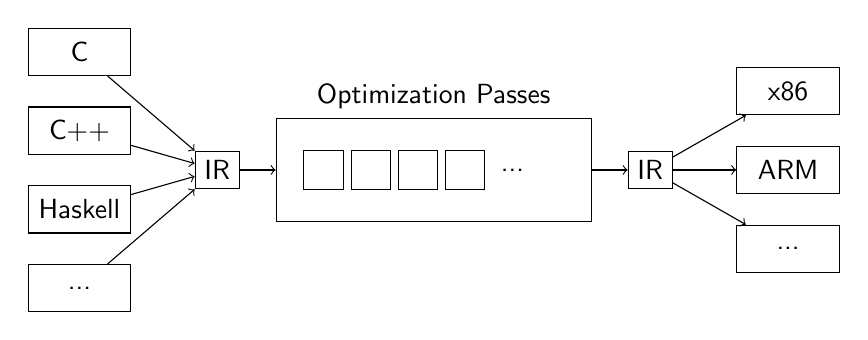
\begin{tikzpicture}
    \node[draw, minimum width=1.3cm, minimum height=0.6cm] at (-2.5,1.5) (C) {C};
    \node[draw, minimum width=1.3cm, minimum height=0.6cm] at (-2.5,0.5) (C++) {C++};
    \node[draw, minimum width=1.3cm, minimum height=0.6cm] at (-2.5, -0.5) (Haskell) {Haskell};
    \node[draw, minimum width=1.3cm, minimum height=0.6cm] at (-2.5, -1.5) (otherl) {...};
    \node[draw] at (-0.75, 0) (irl) {IR};
    
    \node[draw, label=Optimization Passes, minimum width=4cm, minimum height=1.3cm] at (2,0) (optimization) {};
    \node[draw, minimum size=0.5cm] at (0.6,0) {};
    \node[draw, minimum size=0.5cm] at (1.2,0) {};
    \node[draw, minimum size=0.5cm] at (1.8,0) {};
    \node[draw, minimum size=0.5cm] at (2.4,0) {};
    \node at (3.0, 0) {...};

    \node[draw] at (4.75, 0) (irr) {IR};
    \node[draw, minimum width=1.3cm, minimum height=0.6cm] at (6.5,1) (x86) {x86};
    \node[draw, minimum width=1.3cm, minimum height=0.6cm] at (6.5,0) (arm) {ARM};
    \node[draw, minimum width=1.3cm, minimum height=0.6cm] at (6.5,-1) (otherr) {...};

    \draw[->] (C) -- (irl);
    \draw[->] (C++) -- (irl);
    \draw[->] (Haskell) -- (irl);
    \draw[->] (otherl) -- (irl);

    \draw[->] (irl) -- (optimization);
    \draw[->] (optimization) -- (irr);

    \draw[->] (irr) -- (x86);
    \draw[->] (irr) -- (arm);
    \draw[->] (irr) -- (otherr);
  \end{tikzpicture}
  \caption{The general architecture of the \llvm{} compiler}
  \label{fig:llvm}
\end{figure}

\subsection{\qemu{}}
\label{sec:qemu}
\qemu{} is a generic and open source machine emulator and virtualizer.\cite{bellard2005qemu}
While it can be used as a full fledged virtualization environment and sandbox, all I need is its ability to run machine code for different architectures.
\qemu{} achieves high emulation speeds by translating the machine code of the emulated system (guest machine) into machine code that the system running \qemu{} (host machine) can understand, instead of simulating a guest machine CPU directly.
This translation is done by the Tiny Code Generator (TCG).
While this translation is exactly the opposite of what I would want, \qemu{} can be compiled with an optional feature called the TCG interpreter (TCI).
This interpreter runs all operations on a simulated CPU, and thus allows me to examine the results for ``balancedness''.
Like using the \llvm{} compiler, using \qemu{} makes any evaluation mechanism I create for it applicable to any desired target platform.

\section{Intended Approach}
\label{sec:methodology}
In this section I will explain in more detail the main parts of my thesis:
\begin{itemize}
\item Finding a balanced arithmetic suitable for all arithmetic and logic operations present in \llvm{} IR.
\item Implementing a transformation of regular IR operations into above representation.
\item Evaluating the arithmetic for balancedness of all intermediate results using \qemu{}.
\end{itemize}

\subsection{Finding a suitable arithmetic}
There are many different ways to balance an 8-bit value in a 32 bit word.
The most naive variant is probably balancing the bits directly, as in \Cref{fig:bit}.
However, this is also the variant that creates the most overhead for conversion and operations on it.
Much nicer to work with is the variant in \Cref{fig:byte}, as the balancing part is cleanly separated from the actual data.


\begin{figure}[h]
  \centering
  \begin{subfigure}{.49\linewidth}
    \centering
    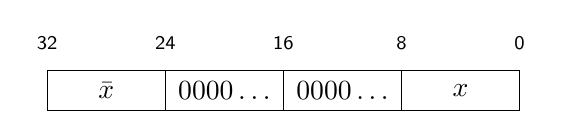
\begin{tikzpicture}
      \node[minimum width=1.5cm, minimum height=0.5cm, draw] at (-2.25, 0) {$\bar{x}$};
      \node[minimum width=1.5cm, minimum height=0.5cm, draw] at (-.75, 0) {$0000\dots$}; 
      \node[minimum width=1.5cm, minimum height=0.5cm, draw] at (0.75, 0) {$0000\dots$}; 
      \node[minimum width=1.5cm, minimum height=0.5cm, draw] at (2.25, 0) {$x$};

      \foreach \x in {0, 8, ..., 32}{
        \node at (3-0.1875*\x, 0.6) {\scriptsize{\x}};
      }
    \end{tikzpicture}
    \caption{Balancing the byte}
    \label{fig:byte}
  \end{subfigure}
  \begin{subfigure}{.49\linewidth}
    \centering
    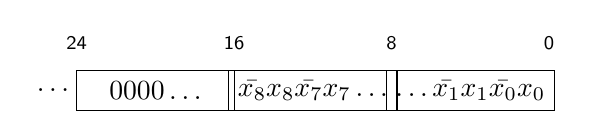
\begin{tikzpicture}
      \node at (-2.3, 0) {$\dots$};
      \node[minimum width=2cm, minimum height=0.5cm, draw] at (-1, 0) {$0000\dots$}; 
      \node[minimum width=2cm, minimum height=0.5cm, draw] at (1, 0) {$\bar{x_8}x_8\bar{x_7}x_7\dots$}; 
      \node[minimum width=2cm, minimum height=0.5cm, draw] at (3, 0) {$\dots\bar{x_1}x_1\bar{x_0}x_0$};

      \foreach \x in {0, 8, ..., 24}{
        \node at (4-0.25*\x, 0.6) {\scriptsize{\x}};
      }
    \end{tikzpicture}
    \caption{Balancing the bits directly}
    \label{fig:bit}
  \end{subfigure}
  \caption{Balancing Schemes}
  \label{fig:schemes}
\end{figure}

The largest problem of using balanced values is that no operation in the ALU will work on them anymore.
This means that I have to find ways to execute all arithmetic and logic operations while keeping the number of unbalanced intermediate values to a minimum.
The simplest way to implement this would be lookup tables, but the size these would require makes this impossible, especially for embedded applications.
A lookup table for 8 bits of data would contain $2^8\cdot2^8=65536$ entries, but this would have unbalanced indices, and require extraction of the unbalanced values before the lookup.
To avoid this the table would need $2^{16}\cdot2^{16}$ entries or 4.2GB of memory, making lookup tables unusable.

So I will have to try and find a chain of intermediate steps to calculate all operations of the \llvm{} IR without creating unbalanced intermediate values.
While this may not entirely be possible, at least a decrease in unbalanced values can be achieved.
Even if the intermediate values are not completely balanced, the distribution of their power consumption might be narrower than that of a regular result.
I have created an evaluation framework for this, and preliminary results show that this is indeed the case.

\subsection{Implementing the optimization pass}
Once I have found a (more) balanced chain of operations for each \llvm{} IR operation, I can create the optimization pass.
Writing the pass should not be too large of a problem, as there are a number of resources for this, and the process is well documented.
The naive version will simply have to traverse all original operations and exchange them for their balanced replacements.

Writing a pass that balances the operations without sacrificing all performance will be harder.
I will have to see how well my custom pass works together with the performance optimization passes built into \llvm{}, both for security and performance.
This will require testing the balancedness for different configurations and orders of the \llvm{} optimization process.

\subsection{Evaluating using \qemu{}}
This part already has a working first version.
I added evaluation code to the optional TCI (see \Cref{sec:qemu}) feature of \qemu{}.
This code logs the operation, the register, the value, and whether or not the value is balanced to a file.
As an absolute count, this is completely sufficient.
However, in order to debug my optimization pass and to have some more contextual information I might also be interested in the actual Assembly and the more high level call stack.
This information can be extracted by moving the evaluation to a GDB (or the \llvm{} alternative LLDB) script, which can attach to the GDB-server stub that \qemu{} provides.
By using such a script I could also output the C and Assembly code, as well as the actual addresses the guest system uses.
By logging data from the TCI evaluating the address bus becomes harder, as the TCI works with host memory directly.
However, running larger programs through a GDB script and evaluating registers at every Assembly instruction will probably be too slow, which is why I started with the TCI version.

For now, the current evaluation code is sufficient and provides enough mechanisms to check the data bus and registers for unbalanced values.

\section{Possible Difficulties}
\label{sec:difficulties}
Finding replacements for all operations will be the most difficult part of this thesis.
As I want to minimize the number of unbalanced intermediate results, I might have to switch between different balancing schemes depending on the operation or location of the data.
Correctness of the new operations will also be an issue.
I will need to prove the correctness of the transformations to and from the balanced representation, as well as for all operations.
However, if no single transformation compromises correctness, neither will the collection of all transformations.

The optimization pass also has potential for problems, as the performance impact of the transformations can prove to be too prohibitive.
If that is the case I need to find a way to either make my balancing work with the existing optimizers of \llvm{} or implement some optimization strategies myself.

The most difficult part of creating the evaluation code will probably remain getting my bearings in the \qemu{} code base, but that has already happened.
By now I have an understanding of the threading model and general architecture of the project, and I am confident I can add any required modifications in a reasonable amount of time.

\section{Related Work}
\label{sec:related-work}
The only paper applying defensive techniques in the compiler itself is by Junod et al.\cite{junod2015obfuscator}.
They integrate a number of software obfuscation techniques, as well as software integrity checks into \llvm{} as optimization passes.
Their approach is very close to my master thesis, however the goal is entirely different.
Junod et al. work on defending programs against reverse engineering and tampering at runtime.
Some of their passes are available online, so that can be used as a tutorial for more complex passes with more interaction with high level data structures like the syntax-tree and the control-flow-graph.

Another paper that works very closely with both \llvm{} and \qemu{} is Lyu et al.\cite{lyu2014dbill}.
They combine the \llvm{} optimizer with \qemu{} to extend static analysis tools utilizing the \llvm{} IR to different target architectures, enabling powerful desktop machines to run the analysis instead of small embedded devices.

\section{Conclusion}
\label{sec:conclusion-schedule}
If successful and without prohibitive performance impacts my thesis would allow generating binaries that are hardened against power analysis, and that for many different platforms.
Even if not, future research on this topic can provide more security for any embedded developer, even without the knowledge needed to incorporate masking schemes and other defensive mechanisms.
I believe that security needs more frameworks along the lines of OpenMP\cite{dagum1998openmp}, to help programmers without security knowledge write secure programs, and that this thesis would be a step in the right direction.

\bibliographystyle{plain}
\bibliography{sources.bib}
\end{document}
